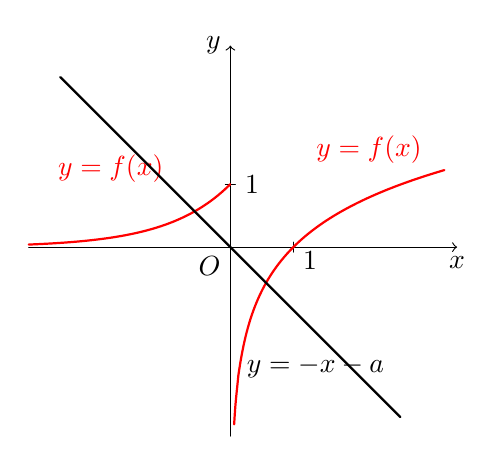
\begin{tikzpicture}[line cap=round,line join=round,scale=0.8]
\usetikzlibrary{calc}

% --- axes ---
\draw[->] (-3.2,0) -- (3.6,0) node[below] {$x$};
\draw[->] (0,-3.0) -- (0,3.2) node[left] {$y$};
\node[below left] at (0,0) {$O$};

% ticks/labels (match the sketch: mark y=1 and x=1)
\draw (-0.08,1) -- (0.08,1) node[right] {$1$};
\draw (1,-0.08) -- (1,0.08) node[below right] {$1$};

% --- red piecewise f(x): e^x (x<=0) and ln x (x>0) ---
\draw[red,thick,smooth,samples=160,domain=-3.2:0]
  plot (\x,{exp(\x)});
\draw[red,thick,smooth,samples=200,domain=0.06:3.4]
  plot (\x,{ln(\x)});

\node[red] at (-1.9,1.25) {$y=f(x)$};
\node[red] at (2.2,1.55) {$y=f(x)$};

% --- line y = -x - a (take a=0 for the picture-style schematic) ---
% so the line crosses (0,0) and has slope -1
\draw[thick] (-2.7,2.7) -- (2.7,-2.7);
\node at (1.35,-1.9) {$y=-x-a$};

\end{tikzpicture}